%%%%%%%%%%%%%%%%%%%%%%%%%%%%%%%%%%%%%%%%%%%%%%%%%%%%%%%%%%%%%%%
%         Estudio empírico de las funciones de activación
%%%%%%
%   1. Comparativas en cuanto a coste computacional.
%%%%%%%%%%%%%%%%%%%%%%%%%%%%%%%%%%%%%%%%%%%%%%%%%%%%%%%%%%%%%%%

\chapter{Funciones de activación}

Como se observó en 
% TODO referencia a que no hay idoneidad a nivel teórico 
% sobre una función de 
se desconoce teóricamente si una función de activación va a ser 
mejor que otra, es por ello y puesto que nuestro objetivo 
es reducir el coste computacional de una red neuronal
que procederemos a realizar un análisis del costo de las redes neuronales. 


\section{Caracterización de las funciones de activación}  

Si bien por conveniencia teórica definimos las funciones de activación en \ref{def:funcion_activacion_articulo}
como una función de $\phi:\R \longrightarrow [0,1]$, no 
decreciente, con uno como límite en infinito y cero como límite a 
menos infinito. 

Nos basaremos en el concepto actual de función de activación,
basta con que sea una función no polinómica
(véanse  los artículos \cite{DBLP:journals/corr/SonodaM15}, \cite{modern-trainable-activation-functions} y \cite{FUNAHASHI1989183}),
además también incluiremos la función de activación identidad.

Funciones no polinómicas hay infinitas y reincidimos en que a priori no hay una mejor que otra; por tanto, como criterio de selección nos guiaremos por la intuición que nos brinda la demostración del teorema \ref{teorema:2_3_uniformemente_denso_compactos}.
  La imagen de una función de activación es relevante a la hora de aproximar la función ideal desconocida, ya que reduce el número 
  de neuronas si se usa convenientemente.  
Por lo tanto, una buena heurística sería disponer de un repertorio básico de funciones de activación que contemplen distintas imágenes no polinómicas. 

Además de las propuestas en \ref{def:funcion_activacion_articulo}, 
añadimos a nuestra colección las siguientes. 


\begin{table}[H] 
    \centering  
    \resizebox{\textwidth}{!}{
    \begin{tabular}{| c | c | c | c |}
        \hline
        Nombre & Expresión & Rango imagen  & Gráfica \\
        \hline
        %%%%%%%% Identidad %%%%%%%
        % Nombre: 
        Identidad 
        & %expresión 
        $Id(x) = x$
        & % Rango imagen
        $(-\infty, +\infty)$
        & % Gráfica
        \begin{minipage}{\coeficienteAncho\textwidth}
            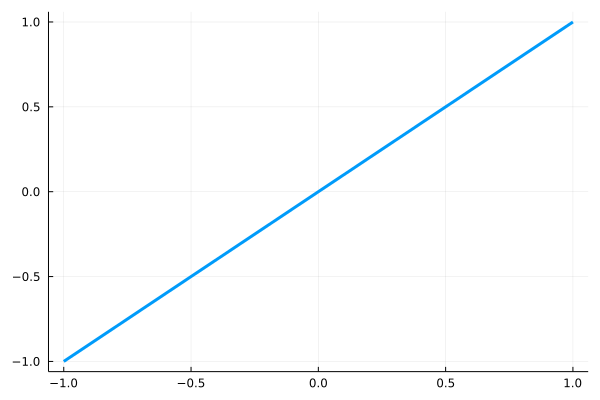
\includegraphics[width=\linewidth]{funciones-activacion/Identidad.png}
        \end{minipage}
        \\
        \hline
         %%%%%%%% Indicadora %%%%%%%
        % Nombre: 
        Indicadora $\lambda \in \R$
        & %expresión 
        $Indicadora_\lambda(x) = 1_{\{x > \lambda\}}$
        & % Rango imagen
        $\{0,1\}$
        & % Gráfica
        \begin{minipage}{\coeficienteAncho\textwidth}
            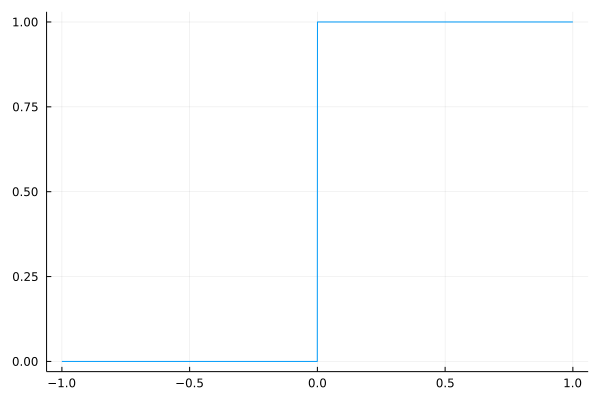
\includegraphics[width=\linewidth]{funciones-activacion/Indicadora de 0.png}
        \end{minipage}
        \\
        \hline
         %%%%%%%% Función umbral %%%%%%%
        % Nombre: 
        Función umbral $p$ polinomio
        & %expresión 
        $Threshold(x) = 1_{\{p(x) > 0\}}$
        & % Rango imagen
        $\{0,1\}$
        & % Gráfica
        \begin{minipage}{\coeficienteAncho\textwidth}
            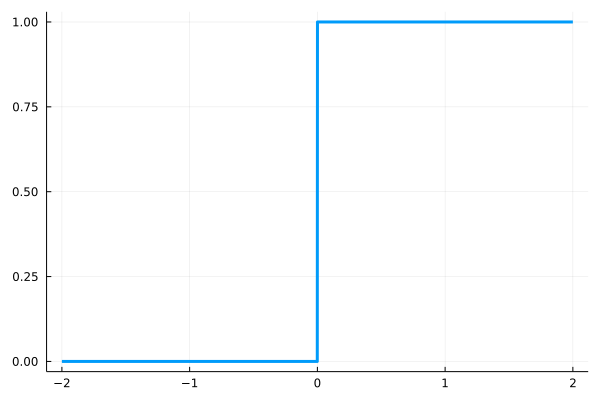
\includegraphics[width=\linewidth]{funciones-activacion/Threshold de polinomio 2x.png}
        \end{minipage}
        \\
        \hline
         %%%%%%%% Función rampa %%%%%%%
        % Nombre: 
        Función rampa
        & %expresión 
        $Rampa(x) = x 1_{\{0 < x <1\}} + 1_{\{x \geq 1\}}$ 
        & % Rango imagen
        $[0,1]$
        & % Gráfica
        \begin{minipage}{\coeficienteAncho\textwidth}
            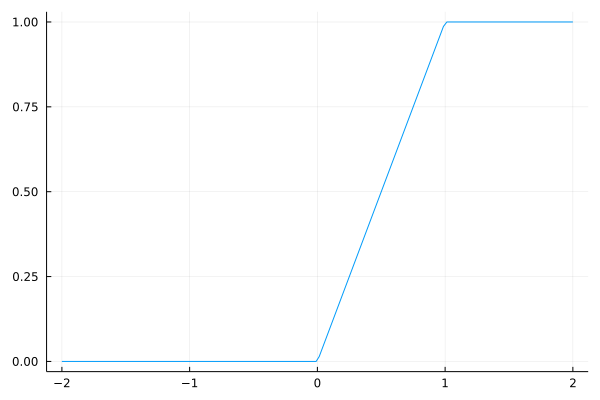
\includegraphics[width=\linewidth]{funciones-activacion/Rampa.png}
        \end{minipage}
        \\
        \hline
        %%%%%%%% sigmoide %%%%%%%%
        % Nombre: 
        Sigmoidea 
        & %expresión 
        $\sigma(x) = \frac{1}{1+e^{-x}}$
        & %Rango imagen
        $(0,1)$
        & % Gráfica
        \begin{minipage}{\coeficienteAncho\textwidth}
            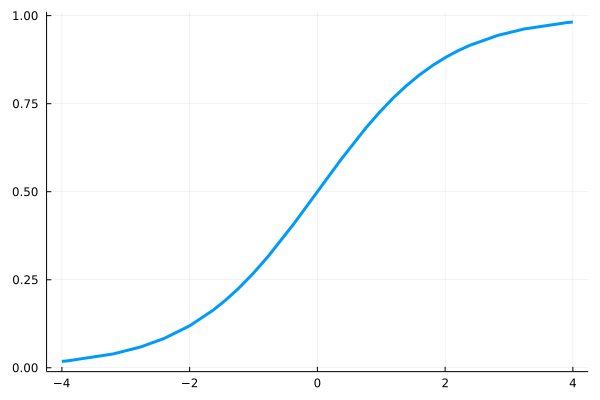
\includegraphics[width=\linewidth]{funciones-activacion/Sigmoid.png}
        \end{minipage}
        \\
        \hline
        %%%%%%%% Tangente hiperbólica  %%%%%%%%
        % Nombre: 
        Tangente hiperbólica 
        & %expresión 
        $\tanh$
        & %Rango imagen
        $(-1,1)$
        & % Gráfica
        \begin{minipage}{\coeficienteAncho\textwidth}
            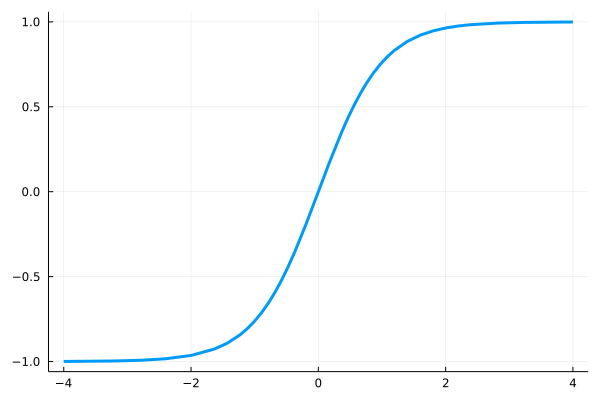
\includegraphics[width=\linewidth]{funciones-activacion/Tangente hiperbolica.png}
        \end{minipage}
        \\
        \hline
        %%%%%%%% Valor absoluto%%%%%%%%
        % Nombre: 
        Valor absoluto
        & %expresión 
        $abs(x)= |x|$
        & %Rango imagen
        $[0,+\infty]$
        & % Gráfica
        \begin{minipage}{\coeficienteAncho\textwidth}
            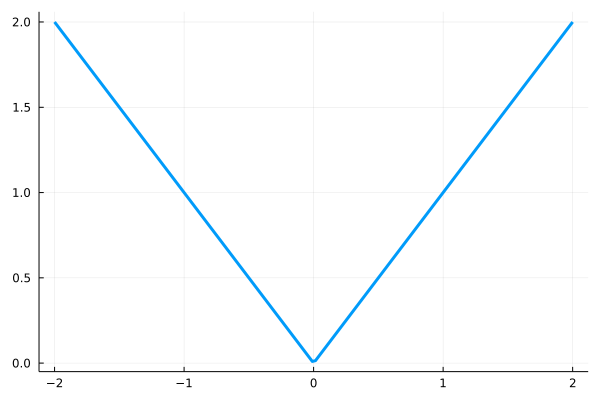
\includegraphics[width=\linewidth]{funciones-activacion/Valor absoluto.png}
        \end{minipage}
        \\
        \hline
         %%%%%%%% Coseno %%%%%%%%
        % Nombre: 
        Coseno
        & %expresión 
        $\cos$
        & %Rango imagen
        $[-1,1]$
        & % Gráfica
        \begin{minipage}{\coeficienteAncho\textwidth}
            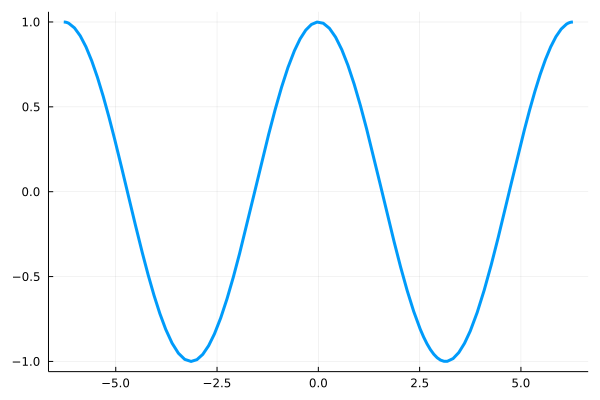
\includegraphics[width=\linewidth]{funciones-activacion/coseno.png}
        \end{minipage}
        \\
        \hline
        %%%%%%%% Cosine Squasher %%%%%%%%
        % Nombre: 
        \textit{Cosine Squasher}
        & %expresión 
        $CosineSquaher(x)=\left(1 + \cos\left(x + 3 \frac{\pi}{2} \right) \frac{1}{2}\right) 
        1_{\{\frac{-\pi}{2} \leq x \leq  \frac{\pi}{2}\}}
        +
        1_{\{ \frac{\pi}{2} < \lambda \}}.$
        & %Rango imagen
        $[0,1]$
        & % Gráfica
        \begin{minipage}{\coeficienteAncho\textwidth}
            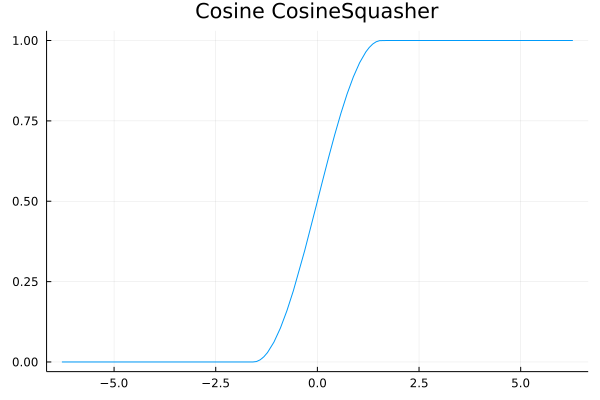
\includegraphics[width=\linewidth]{funciones-activacion/Cosine CosineSquasher.png}
        \end{minipage}
        \\
        \hline
        %%%%%%%% ReLU %%%%%%%%
        % Nombre: 
        \textit{ReLU}
        & %expresión 
        $ReLU(x) = \max(0,x)$
        & %Rango imagen
        $[0,+\infty)$
        & % Gráfica
        \begin{minipage}{\coeficienteAncho\textwidth}
            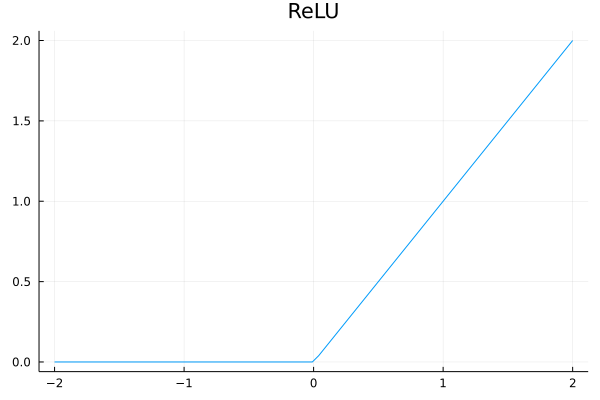
\includegraphics[width=\linewidth]{funciones-activacion/ReLU.png}
        \end{minipage}
        \\
        \hline
        %%%%%%%% Hard Hyperbolic Function %%%%%%%%
        % Nombre: 
        \textit{Hard Hyperbolic Function}
        & %expresión 
        $Hardtanh(x) =\left\{ \begin{array}{lcc}
            -1 &   si  & x \leq -1 \\
            \\ x &  si & -1< x < 1 \\
            \\ 1&  si  & x \geq 1 
            \end{array}
        \right.$
        & %Rango imagen
        $[-1,1]$
        & % Gráfica
        \begin{minipage}{\coeficienteAncho\textwidth}
            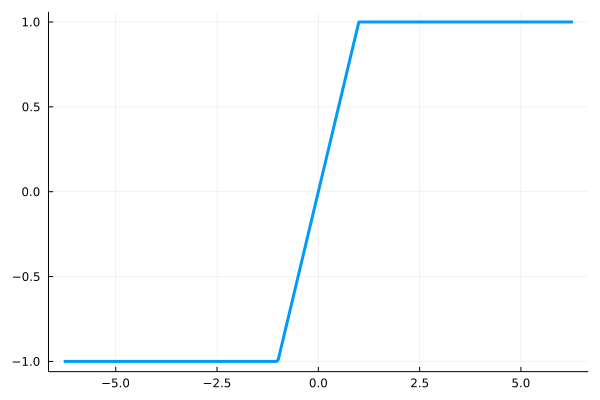
\includegraphics[width=\linewidth]{funciones-activacion/hardtanh.png}
        \end{minipage}
        \\
        \hline
        %%%%%%%% Leaky ReLU%%%%%%%
        % Nombre: 
        \textit{Leaky ReLU}
        & %expresión 
        $\begin{array}{c}

            LReLU_{\alpha}(x) =\left\{ \begin{array}{lcc}
            \alpha x &   si  & x \leq 0 \\
            \\ x&  si  & x > 0 
            \end{array}
            \right.
        \\
        \text{con } \alpha \in \R^+ \text{valor }\textit{pequeño}.
        \end{array}
        $
        & % Rango imagen
        $[0, +\infty)$
        & % Gráfica
        \begin{minipage}{\coeficienteAncho\textwidth}
            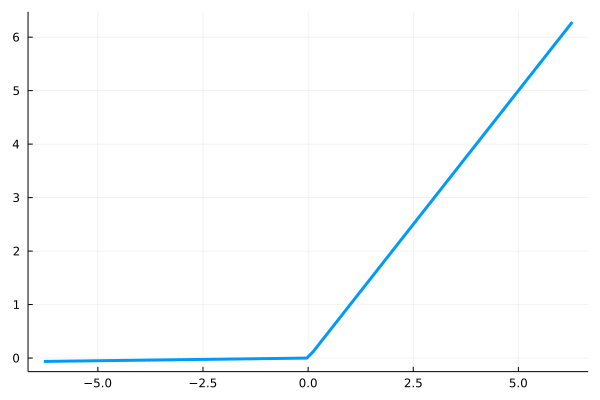
\includegraphics[width=\linewidth]{funciones-activacion/LReLU.png}
        \end{minipage}
        \\
        \hline
    \end{tabular}
    } % fin de llave de ajustarse al ancho de la página
    \caption{Compendio de funciones de activación}  
    \label{table:funciones-de-activation}
\end{table}

\begin{aportacionOriginal}

\begin{teorema}\label{teo:eficacia-funciones-activation}
    Sea $\phi \in \mathcal{A}(\R^2)$ una transformación afín, sean dos funciones de activación $\sigma, \gamma$ tales que 
    \begin{equation*}
        \phi \circ \sigma = \gamma,
    \end{equation*}
    entonces para 
    el espacio de redes neuronales de $n$ neuronas creado con la función de activación $\sigma$ es  
    igual al espacio de redes neuronales creado con la función de activación $\gamma$. 
\end{teorema}
\begin{proof}

    Sea $\mathcal{H}^+_{\sigma, n}(\R^d, \R^s)$, el espacio de redes neuronales con $n$ neuronas con sesgo. 

    Para cualquier $h  \in \mathcal{H}^+_{\sigma, n}(\R^d, \R^s)$
    la proyección i-ésima de $h$ será de la forma 

    \begin{equation*}
        h_i(x) = \sum^n_{j=1}(\beta_{j} \sigma(A_j(x))+ k_j),
    \end{equation*}
    con $x \in \R^d, \beta_{j}, k_j \in \R, A_j \in \afines$. 

    Procedemos a definir $\tilde{h}_i(x)$ como sigue y
    se tiene que 
    \begin{equation*}
        \tilde{h}_i(x) 
        = \sum^n_{j=1}(\beta_{j}  \phi(\sigma(A_j(x)))+ k_j)
        = \sum^n_{j=1}(\tilde{\beta}_{j} \sigma(A_j(x)+ \tilde{k_j})),
    \end{equation*}
    con $x \in \R^d, \tilde \beta_{j}, \tilde k_j \in \R, A_j \in \afines$,
    por lo que está claro que $\tilde{h}_i(x) \in \mathcal{H}^+_{\sigma, n}(\R^d, \R^s)$. 

    Pero por hipótesis del teorema $\phi \circ \sigma = \gamma$, por lo que $\tilde{h}_i(x) \in \mathcal{H}^+_{\gamma, n}(\R^d, \R^s)$. 

    Basta con considerar la transformación afín inversa para ver que
    \begin{equation*}
        \mathcal{H}^+_{\gamma, n}(\R^d, \R^s) = \mathcal{H}^+_{\sigma, n}(\R^d, \R^s).
    \end{equation*}

    Como demostramos en \ref{consideration-irrelevancia-sesgo} se tiene que 
    \begin{equation*}
        \mathcal{H}^+_{\gamma, n}(\R^d, \R^s) \subset \mathcal{H}_{\gamma, n+1}(\R^d, \R^s).
    \end{equation*}
    Por lo que tomando límite cuando $n$ tiende a infinito se tiene lo que buscábamos probar.

    \begin{equation*}
        \mathcal{H}_{\gamma, n}(\R^d, \R^s) = \mathcal{H}_{\sigma, n}(\R^d, \R^s).
    \end{equation*}
\end{proof}
\end{aportacionOriginal}

\subsubsection*{Relevancia práctica del teorema}
Este teorema lo que nos está diciendo es que si dos funciones de activación tienen \textit{la misma forma}
(independientemente de su grafo)
entonces \textbf{aproximarán igual de bien},
es decir, con el mismo error dentro de un conjunto de datos.
 Esto a nivel práctico  significa que \textbf{si se tienen dos funciones de activación
  \textit{con la misma forma} (o muy parecidas) elige
   la que tenga menor costo computacional}, porque a 
   nivel teórico aproximarán igual de bien y de esta
    manera ahorraremos recursos. 

Notemos además que la demostración nos enseña que la igualdad se da independientemente del número de 
neuronas fijado, es decir que no es un resultado 
asintótico (lo asintótico en términos prácticos 
significa que sea resultado de una serie de 
aproximaciones).  


Así pues a la vista de la imágenes de las distintas funciones de activación 
recogidas en la tabla \ref{table:funciones-de-activation} y
por el recién probado teorema \ref{teo:eficacia-funciones-activation} podemos determinar a priori que de manera teórica existen conjuntos de funciones que aproximadamente  puedes producir los mismos resultado, 
compararemos entonces su coste computacional y tomaremos como representante de la clase aquel que sea de menor coste. 

\begin{table}[H] 
    \centering  
    \begin{tabular}{| c | c | c | }
        \hline
        Indicadora &  Rampa & ReLU \\
        Umbral & Sigmodea & LReLU\\
        & \textit{Cosine Squasher}& \\
        & tanh& \\
        & \textit{Hard Hyperbolic Function}& \\
\hline
    \end{tabular}
    \caption{Clases de equivalencia de funciones de activación}  
    \label{table:Clases-equivalencia-activation-function}
\end{table}


